%Preamble
\documentclass[12pt]{article}
\usepackage{fancyhdr}
\usepackage{extramarks}
\usepackage{amsmath}
\usepackage{amssymb}
\usepackage{amsthm}
\usepackage{amsrefs}
\usepackage{amsfonts}
\usepackage{mathrsfs}
\usepackage{mathtools}
\usepackage[mathcal]{eucal} %% changes meaning of \mathcal
\usepackage{enumerate}
\usepackage[shortlabels]{enumitem}
\usepackage{verbatim} %% includes comment environment
\usepackage{hyperref}
\usepackage[capitalize]{cleveref}
\crefformat{equation}{~(#2#1#3)}
\usepackage{caption, subcaption}
\usepackage{graphicx}
\usepackage{fullpage} %%smaller margins
\usepackage[all,arc]{xy}
\usepackage{mathrsfs}

\hypersetup{
    linktoc=all,     % set to all if you want both sections and subsections linked
}

\topmargin=-0.45in
\evensidemargin=0in
\oddsidemargin=0in
\textwidth=6.5in
\textheight=9.0in
\headsep=0.25in
\setlength{\headheight}{16pt}

\linespread{1.0}

\pagestyle{fancy}
\lhead{\Name}
\chead{\hwClass: \hwTitle}
\rhead{\hwDueDate}
\lfoot{\lastxmark}
\cfoot{\thepage}

\renewcommand\headrulewidth{0.4pt}
\renewcommand\footrulewidth{0.4pt}

\setlength\parindent{0pt}

%% Title Info
\newcommand{\hwTitle}{HW \# 6}
\newcommand{\hwDueDate}{March 10, 2021}
\newcommand{\hwClass}{AMATH 585}
\newcommand{\hwClassTime}{}
\newcommand{\hwClassInstructor}{}
\newcommand{\Name}{\textbf{Marlin Figgins}}


%% MATH MACROS
\newcommand{\bbF}{\mathbb{F}}
\newcommand{\bbN}{\mathbb{N}}
\newcommand{\bbQ}{\mathbb{Q}}
\newcommand{\bbR}{\mathbb{R}}
\newcommand{\bbZ}{\mathbb{Z}}
\newcommand{\bbC}{\mathbb{C}}
\newcommand{\abs}[1]{ \left| #1 \right| }
\newcommand{\diff}[2]{\frac{d #1}{d #2}}
\newcommand{\infsum}[1]{\sum_{#1}^{\infty}}
\newcommand{\norm}[1]{ \left|\left| #1 \right|\right| }
\newcommand{\eval}[1]{ \left. #1 \right| }
\newcommand{\Expect}[1]{\mathbb{E}\left[#1 \right]}
\newcommand{\Var}[1]{\mathbb{V}\left[#1 \right]}
\renewcommand{\vec}[1]{\mathbf{#1}}

\renewcommand{\phi}{\varphi}
\renewcommand{\emptyset}{\O}

%--------Theorem Environments--------
%theoremstyle{plain} --- defaultx
\newtheorem{thm}{Theorem}[section]
\newtheorem{cor}[thm]{Corollary}
\newtheorem{prop}[thm]{Proposition}
\newtheorem{lem}[thm]{Lemma}
\newtheorem{conj}[thm]{Conjecture}
\newtheorem{quest}[thm]{Question}

\theoremstyle{definition}
\newtheorem{defn}[thm]{Definition}
\newtheorem{defns}[thm]{Definitions}
\newtheorem{con}[thm]{Construction}
\newtheorem{exmp}[thm]{Example}
\newtheorem{exmps}[thm]{Examples}
\newtheorem{notn}[thm]{Notation}
\newtheorem{notns}[thm]{Notations}
\newtheorem{addm}[thm]{Addendum}

% Environments for answers and solutions
\newtheorem{exer}{Exercise}
\newtheorem{sol}{Solution}

\theoremstyle{remark}
\newtheorem{rem}[thm]{Remark}
\newtheorem{rems}[thm]{Remarks}
\newtheorem{warn}[thm]{Warning}
\newtheorem{sch}[thm]{Scholium}

\makeatletter
\let\c@equation\c@thm
\makeatother

\begin{document}
\begin{exer}
The conjugate gradient method for solving a symmetric positive definite linear system
$Ax=b$ can be written as below:
\vspace{.1in}

\begin{center}
\begin{tabular}{|l|} \hline
Given $x_0$, compute $r_0 = b - A x_0$, and set $p_0 = r_0$. \\
For $k=1,2, \ldots$, \\
$~~$ Compute $A p_{k-1}$. \\
$~~$ Set $x_k = x_{k-1} + a_{k-1} p_{k-1}$, where $a_{k-1} = \frac{\langle r_{k-1} , r_{k-1} \rangle}
{\langle p_{k-1} , A p_{k-1} \rangle}$. \\
$~~$ Compute $r_k = r_{k-1} - a_{k-1} A p_{k-1}$. \\
$~~$ Set $p_k = r_k + b_{k-1} p_{k-1}$, where $b_{k-1} = \frac{\langle r_k , r_k \rangle}
{\langle r_{k-1} , r_{k-1} \rangle}$. \\
Endfor \\ \hline
\end{tabular}
\end{center}
\vspace{.1in}

\begin{enumerate}[(a)]
\item
Show that the residual vectors $r_0 , \ldots , r_k$ are orthogonal to each other
($\langle r_i , r_j \rangle = 0$ if $i \neq j$) and that the direction vectors 
$p_0 , \ldots , p_k$ are $A$-orthogonal ($\langle p_i , A p_j \rangle = 0$ if $i \neq j$).
[Hint:  First show that $\langle r_1 , r_0 \rangle = \langle p_1 , A p_0 \rangle = 0$
and then use induction on $k$.]

\item
If $A$ is the $N \times N$ matrix of the 5-point operator for Poisson's equation on a square,
count the number of operations (additions, subtractions, multiplications, and divisions) performed
in each iteration.  (Show how you arrive at your result.)

\item
Compare your operation count in (b) to that of a Gauss-Seidel iteration applied to the
same $N$ by $N$ 5-point matrix $A$.  Also compare to the operation count for a multigrid 
V-cycle, using one Gauss-Seidel iteration on each visit to each grid level.
(Again, show how you derive your operation counts.)
\end{enumerate}
\end{exer}

\begin{sol}
    (a) We'll begin with the base case. Starting with
    \begin{align*}
        (r_{1}, r_{0}) &= (r_{0}, r_{0}) - a_{0} (A p_{0}, r_{0})\\
                       &= (r_{0}, r_{0}) - \left(\frac{(r_{0}, r_{0})}{(p_{0}, A p_{0})}\right) (A p_{0}, r_{0}) \\
                       &= 0,
    \end{align*}
    where in the last line we've used that $p_{0} = r_{0}$. Next, we have that
    \begin{align*}
        (p_{1}, A p_{0}) &= (r_{1}, A p_{0}) + b_{0} (p_{0}, A p_{0})\\
                         &= (r_{1}, a_{0}^{-1}(r_{0} - r_{1})) + b_{0} (r_{0}, a_{0}^{-1}(r_{0} - r_{1}))\\
                         &= -(r_{1}, a_{0}^{-1}r_{1}) + a_{0}^{-1}b_{0} (r_{0}, r_{0} )\\
                         &= 0,
    \end{align*}
    where we've used that $Ap_{0} = a_{0}^{-1}(r_{0} - r_{1})$, $(r_{1}, r_{0}) = 0$, and the definition of $b_{0}$. We'll now assume that the following is true for all $i < k$,
    \begin{align*}
        (r_{k}, r_{i}) = (p_{k}, A p_{i} ) = 0.
    \end{align*}
    We can then write 
    \begin{align*}
        (p_{k}, Ap_{k}) &= (r_{k}, Ap_{k}) + b_{k-1} (p_{k-1}, A p_{k})\\
                        &= (r_{k}, A p_{k}) + b_{k-1}(A p_{k-1}, p_{k})\\
                        &= (r_{k}, A p_{k})
    \end{align*}
    since $A$ is real symmetric. This allows us to show
    \begin{align*}
        (r_{k+1}, r_{k}) &= (r_{k}, r_{k}) - a_{k} (A p_{k}, r_{k}) \\
                         &= (r_{k}, r_{k}) - \left(\ \frac{(Ap_{k}, r_{k})}{(A p_{k}, p_{k})}  \right) (r_{k}, r_{k}) = 0.
    \end{align*}
    Additionally, we have that
    \begin{align*}
        (r_{k}, p_{k}) &= (r_{k}, r_{k}) + b_{k-1} (r_{k}, p_{k-1})\\
                       &= (r_{k}, r_{k}) + b_{k-1} (r_{k}, r_{k-1}) + b_{k-1}b_{k-2}(r_{k}, p_{k-2})+ \cdots \\
                       &= (r_{k}, r_{k}),
    \end{align*}
    as we continue this pattern of reducing $p_{k} = r_{k} + b_{k-1} p_{k-1}$, we will get terms of the form $(r_{k}, r_{j}) = 0$ and $(r_{k}, p_{j})$ until we reach $(r_{k}, p_{0}) = (r_{k}, r_{0}) = 0$. We'll pair this with the following
    \begin{align*}
        (r_{k+1}, p_{k}) = (r_{k}, p_{k}) - a_{k} (A p_{k}, p_{k}) = 0.
    \end{align*}
    These two equalities allow us to show that
    \begin{align*}
        (Ap_{k}, p_{k+1}) &= (Ap_{k}, r_{k+1}) + \frac{(r_{k+1}, r_{k+1})}{(r_{k}, r_{k})} (A p_{k}, p_{k})\\
                          &= (a^{-1}_{k}(r_{k} - r_{k+1}), r_{k+1}) +  \frac{(r_{k+1}, r_{k+1})}{(r_{k}, r_{k})} \left[  (a^{-1}_{k}(r_{k} - r_{k+1}), p_{k}) \right]\\
                          &= -a_{k}^{-1}(r_{k+1}, r_{k+1}) + a_{k}^{-1}(r_{k+1}, r_{k+1}) = 0.
    \end{align*}
We've therefore shown
\begin{align*}
    (Ap_{k}, p_{k+1}) = (r_{k+1}, r_{k}) = 0.
\end{align*}
We then have that
\begin{align*}
    (r_{k+1}, r_{j}) &= (r_{k}, r_{k}) - a_{k} (Ap_{k}, r_{j})\\ 
                     &= - a_{k} (p_{k}, A [p_{j} - b_{j-1}p_{j-1}]) = 0
\end{align*}
Lastly, 
\begin{align*}
    (p_{k+1}, A p_{j}) &= (r_{k+1}, Ap_{j}) + b_{k}(p_{k}, Ap_{j})\\
                       &= (r_{k+1}, a_{j}^{-1}(r_{j} - r_{j+1}) = 0,
\end{align*}
which completes the proof.

(b) We'll start with some baseline groundwork. Each inner product computed (assuming we add any zeros anyway) will typically result in $N$ multiplications (for each index) and $N - 1$ additions. Starting $A p_{k-1}$, computing the product in each row requires $5$ multiplications and $4$ additions for each of the $N$ rows. Therefore,  $A p_{k-1}$ requires $5N$ multplications and $4N$ additions. 
\begin{align*}
    +: 4(N-1), \quad  \times: 5N
\end{align*}

We then must compute $a_{k-1}$ which requires computing two inner products of known values and one division
\begin{align*}
    +: 4(N-1)  + 2(N-1) = 6(N-1), \quad  \times: 5N + 2N = 7N, \quad \div: 1
\end{align*}

Multiplying $p_{k-1}$ by $a_{k-1}$ is scalar multiplication and requires $N$ multiplications 
\begin{align*}
    +: 6(N-1), \quad  \times: 7N + N = 8N, \quad \div: 1
\end{align*}

Adding $x_{k+1} + a_{k-1} p_{k-1}$ requires $N$ additions
\begin{align*}
    +: 6(N-1) + N = 7N - 6, \quad  \times: 8N, \quad \div: 1
\end{align*}

To compute $r_{k}$, we'll need $N$ subtractions and $N$ multiplications
\begin{align*}
+: 7N - 6, \quad  \times: 8N + N = 9N, \quad \div: 1, \quad -: N.
\end{align*}

For $b_{k-1}$, we compute two inner products and divide once
\begin{align*}
    +: 7N - 6  + 2(N-1) = 9N - 7, \quad  \times: 9N + 2N = 11N, \quad \div: 1 + 1 = 2, \quad -: N.
\end{align*}
To compute $p_{k}$, we need $N$ additions and $N$ multiplications
\begin{align*}
    +: 9N - 7 + N = 10N - 7, \quad  \times: 11N + N = 12N, \quad \div: 1 + 1 = 2, \quad -: N.
\end{align*}
This gives $\approx23N$ operations for each loop of conjugate gradient.

(c) We'll now do the operator count for each iteration of Gauss-Seidel. First, we set $M$ to be the lower triangle of the matrix. We also define $N = U$, the strict upper triangle of $A$.  The rest of the loop is given by
\begin{align*}
    M u^{(k+1)} &= N u^{(k)} + f,
\end{align*}
where we solve for $u$ using forward substitution, so that
\begin{align*}
    u^{(k+1)}_{i} = \frac{1}{a_{ii}} \left(f_{i} - \sum_{j=1}^{i-1} a_{ij}  u^{(k+1)}_{i}  - \sum_{j=i+1}^{n} a_{ij} u_{j}^{(k)}\right).
\end{align*}
As the matrix $A$ has only 5 non-zero elements per row, we have that there are $5$ multiplications, $5$ subtractions, and $1$ division per row
\begin{align*}
    +: 0, \quad  \times: 5N, \quad \div: N, \quad -: 5N.
\end{align*}
For a $V$ cycle using one Gauss-Seidel iteration, we have that if there are $n$ layers for which the size decreases by $1 / 2$ per layer. And smoothing occurs once at each visit (of which there are two to each layer), we have that total operations from follow the GS step alone
\begin{align*}
    \text{Op}_{G}(N) =  2 \cdot \sum_{k = 0}^{n} \left(11\frac{N}{2^{k}}\right) \approx 44N,
\end{align*}
where $N$ is the size of the largest grid. We use an approximation large $n$ to get an estimate of $44N$. At each step, we must also project or interpolate the error which requires (at the highest level) $N$ additions and $N$ divisions for interpolation as we take the average of neighboring points and 0 mathematical operations for projection (we simply take every other element of the finer grid, so there's no need for addition, subtraction, multiplication or division). We then have that as there $n-1$ interpolations on the up cycle to get back to the full grid
 \begin{align*}
     \text{Op}_{IC}(N) = \sum_{k=1}^{n} \left(  2 \frac{N}{2^{k}}    \right) \approx 2N.
\end{align*}

Lastly, we have that we must add the errors accumulated to the final solution which has $N$ additions. This gives a final operations count as
 \begin{align*}
     \text{Op}(N) \approx 44N + 2N + N = 47N
\end{align*}
in the large $n$ limit.
\end{sol}

\newpage

\begin{exer}
Repeat the experiments on p.~103 of the text, leading to Figures 4.8 and
4.9, but use the Gauss-Seidel method and (unpreconditioned) CG instead of
Jacobi iteration.
That is, set up difference equations for the problem
\[
u''(x) = f(x),~~~u(0) = 1 ,~u(1) = 3 ,
\]
where
\[
f(x) = -20 + a \phi'' (x) \cos( \phi (x)) - a ( \phi' (x) )^2 \sin ( \phi (x) ),
\]
where $a = 0.5$ and $\phi (x) = 20 \pi x^3$.  The true solution is
\[
u(x) = 1 + 12 x - 10 x^2 + a \sin ( \phi (x) ) .
\]
Starting with initial guess $u^{(0)}$ with components $1 + 2 x_i$,
$i=1, \ldots , 255$, run, say, $20$ Gauss-Seidel iterations and then
$20$ CG iterations, plotting the true solution to the linear system
and the approximate solution, say, at steps 0, 5, 10, and 20, and
also plotting the error (the difference between true and approximate
solution).  Print the size of the error (the $L_2$-norm or the $\infty$-norm)
at these steps too.  Based on your results, would you say that Gauss-Seidel
and CG would be effective smoothers for a multigrid method?
\end{exer}

\begin{sol}
    I've implemented this all using julia. It appears that for the specified number of steps that Gauss-Seidel and CG both make progress by figuring out the higher frequencies first. Because of this, I think both methods would make effective smoothers for multigrid as the coarse grid operators would be useful for figuring out lower frequencies, leaving little work for GS and CG and allowing faster convergence.

    \begin{figure}[ht]
        \centering
        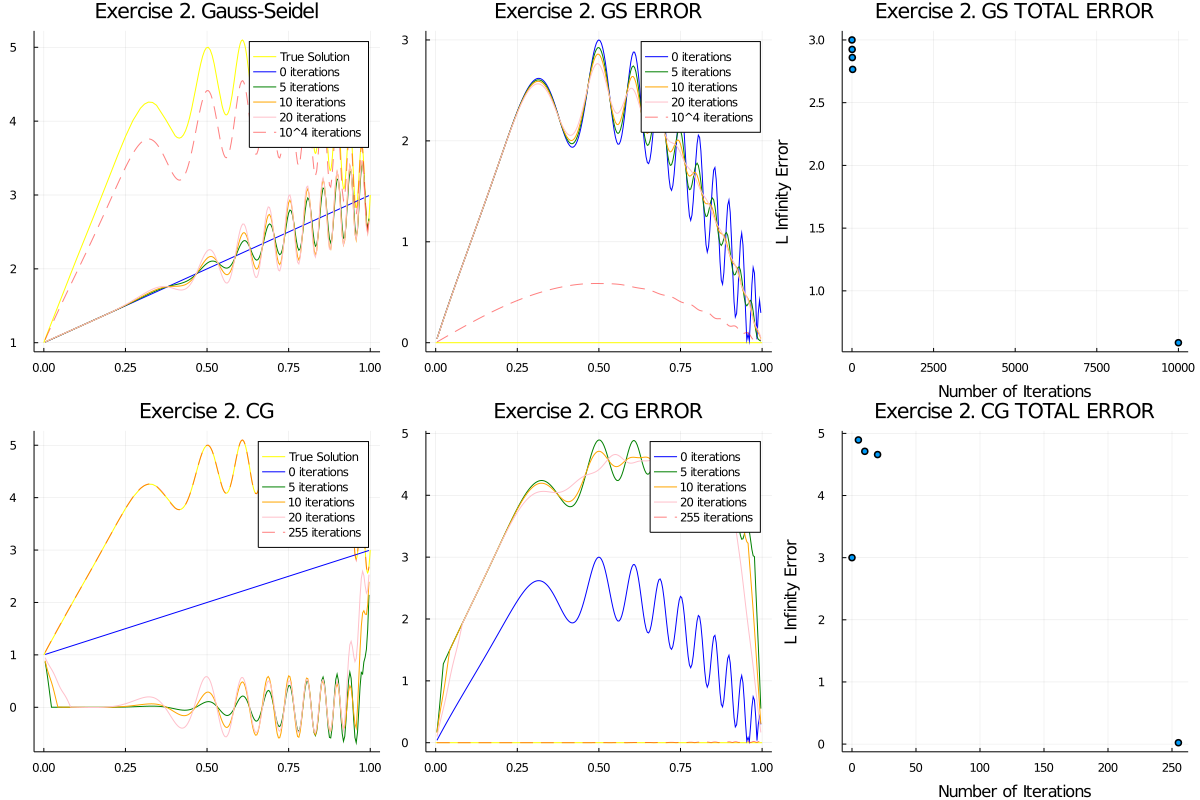
\includegraphics[width=0.8\linewidth]{figs/hw-6-exer-2-gs-cg.png}
        \caption{}%
        \label{fig:Exercise_2}
    \end{figure}
\end{sol}

\newpage

\begin{exer}
Implement a 2-grid method for solving the 1D model problem with homogeneous Dirichlet
boundary conditions:
\[
u_{xx} = f(x) ,~~u(0) = u(1) = 0.
\]
Use linear interpolation to go from the coarse grid with spacing $2h$ to the fine grid
with spacing $h$.  Take the projection matrix $I_h^{2h}$, going from the fine grid to the
coarse grid, to be $0.5$ times the transpose of the interpolation matrix: 
$I_h^{2h} = \frac{1}{2} ( I_{2h}^h )^T$.
Use a multigrid V-cycle with 1 smoothing step on each visit to each grid level. 
Try weighted Jacobi and Gauss-Seidel as the smoothing step.
Try several different values of the mesh spacing $h$ and show that you achieve convergence to
a fixed tolerance in a number of cycles that is independent of the mesh size.
\end{exer}

\begin{sol}
    I've implemented this in Julia using weighted Jacobi smoothing. Code can be found in the appendix. We see that for the fixed tolerance $0.001$. I find that for various grid sizes $M = 150, \ldots, 1000$ and the corresponding $h$ it takes around 5 cycles to converge within the tolerance. For some intermediate $M$ values this goes up to 7 but there doesn't appear to be a strong dependence on the mesh size for the number of cycles needed to reach a fixed tolerance.

    \begin{figure}[ht]
        \centering
        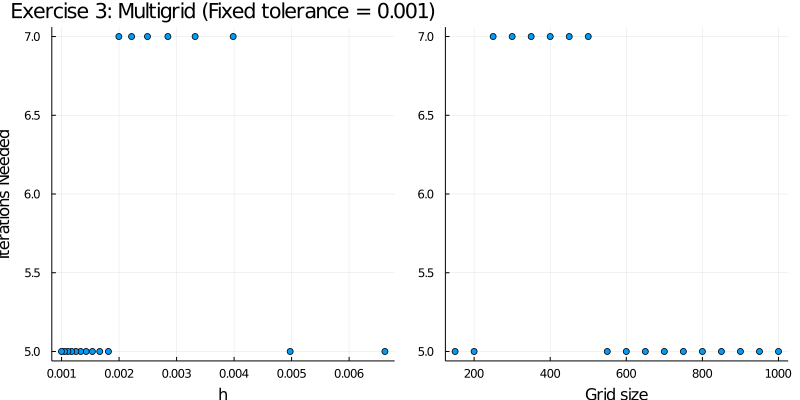
\includegraphics[width=0.8\linewidth]{figs/hw-6-exer-3-multigrid.png}
        \caption{}%
        \label{fig:Exercise_3}
    \end{figure}
\end{sol}

\newpage

\begin{exer}
    \begin{enumerate}[(a)]
\item
Consider an iteration of the form 
\[
x_k = x_{k-1} + M^{-1} ( b - A x_{k-1} ) ,
\]
for solving a nonsingular linear system $Ax=b$.  Note that the error $e_k := A^{-1} b - x_k$
satisfies
\[
e_k = (I - M^{-1} A) e_{k-1} = \ldots = (I - M^{-1} A)^k e_0.
\]
Assume that $\| e_0 \|_2 = 1$ and that $\| I - M^{-1} A \|_2 = \frac{1}{2}$.
Estimate the number of iterations required to reduce the 2-norm of the error below $2^{-20}$.
Show how you obtain your estimate.  Now suppose you know only that the spectral radius
$\rho ( I - M^{-1} A ) = \frac{1}{2}$.  Can you give an estimate of the number of iterations
required to reduce the 2-norm of the error below $2^{-20}$?  Explain why or why not.

\item
Consider the GMRES algorithm applied to an $n$ by $n$ matrix $A$ with the sparsity pattern 
pictured below:
\[
\left[ \begin{array}{ccccc}
\ast & \ast & \cdots & \ast & \ast \\
\ast & \ast & \cdots & \ast & 0 \\
0    & \ast & \cdots & \ast & 0 \\
\vdots  & \ddots & \ddots & \vdots & \vdots \\
0    & \cdots    & \cdots & \ast & 0 \end{array} \right] ,
\]
where the $\ast$'s represent nonzero entries.  Show that if the initial residual is the 
$n$th unit vector $( 0, \ldots , 0 , 1 )^T$, then the algorithm makes no progress
until step $n$.  Show that a matrix with this sparsity pattern can have {\em any}
eigenvalues.  Conclude that eigenvalue information alone cannot be enough to ensure
fast convergence of the GMRES algorithm.
\end{enumerate}
\end{exer}

\begin{sol}
We will bound $e_{k}$ using bounds on $I- M^{-1}A$. We know that \begin{align*}
\norm{e_{k}}_{2} \leq \norm{I - M^{-1} A}_{2} \norm{e_{k-1}}_{2} \leq \norm{I - M^{-1} A}_{2}^{k} \norm{e_{0}}_{2} = 2^{-k}. %TODO:Why do we know this?
\end{align*}
With this estimate, we estimate that the it would take at most $20$ iterations to reach  $2^{-20}$ accuracy. If we only know the spectral radius, the rate of convergence will additionally depend on the condition number of the eigenvalue matrix. We can see this as follows. Assume that we can eigen-decompose $I - M^{-1}A$ as follows
\begin{align*}
(I - M^{-1} A) = R^{-1} \Lambda R^{-1}
\end{align*}

Then we would have that
\begin{align*}
    \norm{e_{k}}_{2} \leq  \norm{\Lambda^{k}}_{2} \norm{R}_{2}\norm{R^{-1}}_{2} \norm{e_{0}}_{2}
\end{align*}
As $\Lambda$ is diagonal, we have that
 \begin{align*}
     \norm{e_{k}}_{2} \leq  \rho^{k} \norm{R}_{2}\norm{R^{-1}}_{2} \norm{e_{0}}_{2} = 2^{-k} \norm{R}_{2}\norm{R^{-1}}_{2},
\end{align*}
so that  $\rho$ alone is not enough enough to make an estimate unless we know  the condition number of  $R$ i.e.  $\kappa(R) = \norm{R}_{2}\norm{R^{-1}}_{2}$.

(b) If $r_0 = q_{1} = e_{n}$, then $A q_{1} = a_{1,n} e_{1}$ where $e_{i}$ is the $i$ unit vector. It then follows that $(v, q_{1}) = h_{11} = 0$ and $q_{2} = e_{1}$. We then have that $v = A q_{2} = a_{1,1} e_{1} + a_{1,2}e_{2}$. We see that for the previous $q_{2}$, $(v, q_{2}) = h_{22} = a_{11}$ and $(v, q_{1}) = h_{21} = 0$, so that $q_{3} = e_{2}$. This process continues with $q_{n} = e_{n-1}$ as $q_{n}$ must be orthogonal to the previous $q_{k}$. This gives the matrix $Q_{k}$ which essentially just a permutation matrix
\begin{align*}
    Q_{k} = [e_{n}, e_{1}, \ldots, e_{k-1}]
\end{align*}
and the Hessenberg matrix $H_{k}$ is also just a swapping of the first $k-1$ columns and the last column of $A$. We then have that
\begin{align*}
r_{k} - r_{0} = - Q_{k+1} H_{k} y_{k}.
\end{align*}
As the first row of the Hesenberg matrix $H_{k}$ is 0 until $k=n$, the least squares solution will return the vector
\begin{align*}
    y_{k} = \min \norm{ \eta - H_{k} y }_{2}
\end{align*}
which is 0 when $\eta$ is defined as 4.72 since the valid solution is all vectors of form $\alpha e_{1}$ and 0 is the least squares among these.

To see this matrix has non-zero eigenvalues, we simply pick constants $\lambda_{i}$ and place them on the open diagonal spot. We then put 1 in the upper right hand corner. This matrix is upper triangular  and will have its eigenvalues be the chosen $\lambda_{i}$. This shows that independent of its eigenvalues a matrix with this sparsity pattern cannot have fast convergence of GMRES, so eigenvalues alone are not alone a determinant of convergence rate.
\end{sol}
\end{document}
